\documentclass[11pt]{article}
\usepackage[a4paper,margin=22mm,headheight=16pt]{geometry}
\usepackage{fontspec,xeCJK,xcolor,graphicx,enumitem,fancyhdr,titlesec}
\usepackage{hyperref}
\IfFontExistsTF{Times New Roman}{\setmainfont{Times New Roman}}{\setmainfont{TeX Gyre Termes}}
\IfFontExistsTF{FangSong}{\setCJKmainfont[AutoFakeBold=2]{FangSong}}{\IfFontExistsTF{仿宋}{\setCJKmainfont[AutoFakeBold=2]{仿宋}}{\IfFontExistsTF{FandolFang-Regular.otf}{\setCJKmainfont[AutoFakeBold=2]{FandolFang-Regular.otf}}{\setCJKmainfont{FandolSong-Regular.otf}}}}
\definecolor{ink}{HTML}{173747}\definecolor{accent}{HTML}{227E82}
\hypersetup{colorlinks=true,urlcolor=accent,linkcolor=accent}
\linespread{1.22}\setlength{\parindent}{0pt}\setlength{\parskip}{6pt}
\setlist[itemize]{leftmargin=1.4em,itemsep=3pt}
\titleformat{\section}{\large\bfseries\color{ink}}{}{0pt}{}
\titlespacing*{\section}{0pt}{14pt}{7pt}
\pagestyle{fancy}\fancyhf{}\lhead{\small OMNI LEARNING / 学习手册}\rhead{\small Source-grounded learning}\cfoot{\small\thepage}
\emergencystretch=2em\widowpenalty=10000\clubpenalty=10000
\newcommand{\Needspace}[1]{\par\begingroup\dimen0=#1\relax\vskip0pt plus\dimen0\penalty-100\vskip0pt plus-\dimen0\vskip\dimen0\penalty9999\vskip-\dimen0\vskip0pt\endgroup}
\begin{document}


{\LARGE\bfseries\color{ink} 希腊柱式与梁柱体系}\par

2026-10-08 | Day02/30 | 阅读 8 分钟 + 练习 3 分钟\par\vspace{6pt}

\Needspace{5\baselineskip}\section*{今日导航}

今天回答：为什么柱式不仅是柱头花样？目标是辨认希腊梁柱体系，并理解柱、梁及上部构件之间的比例关系。先回忆昨日：一张正面照片能回答哪些问题，又缺少哪些信息？

\Needspace{5\baselineskip}\section*{从支撑关系看神庙}

看图 B：竖直立柱支撑水平构件，形成梁柱关系。图示帮助识别基本构成，不是某座神庙的考古复原。石材在不同受力方式下表现不同，水平跨越的构件需要相应尺度和支撑；实际结构分析比这幅简图复杂，今天不做受力计算。

\begin{center}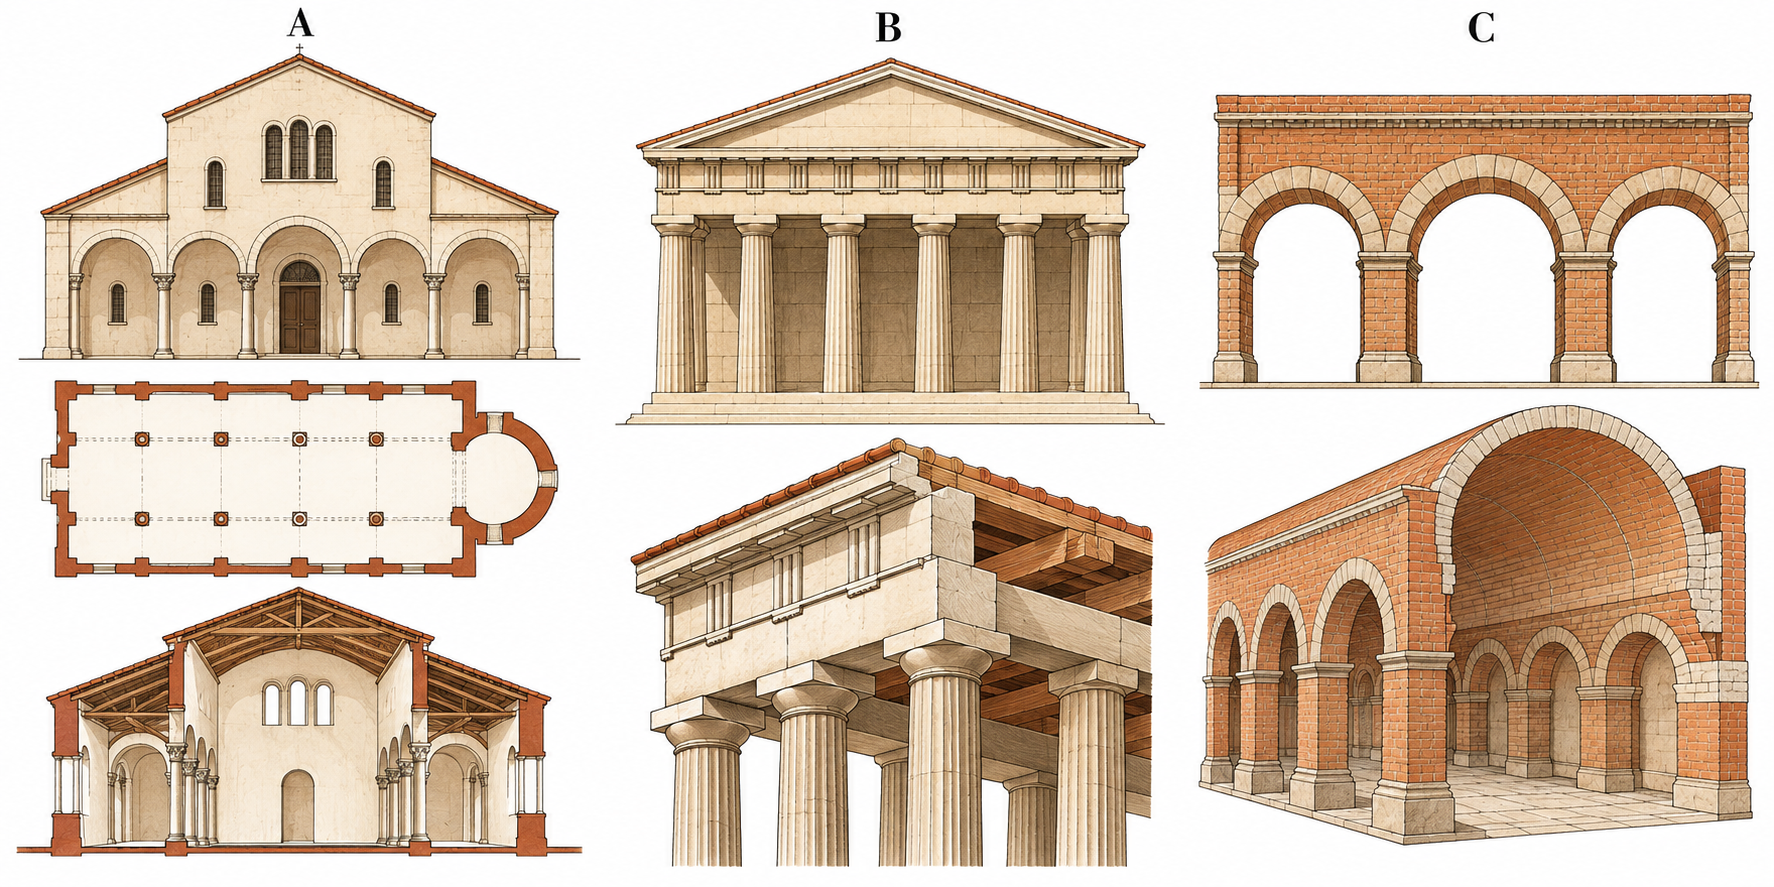
\includegraphics[width=\linewidth,height=0.26\textheight,keepaspectratio]{../assets/figure-9ba448966b26.png}\par

{\small 本课重点看 B 区。A 平面、立面与剖面提供不同信息；B 梁柱；C 拱券与桶形拱顶。图为类型示意，不是具体遗址测绘图。}\par

{\footnotesize AI生成教学示意，非实物照片、原始史料或官方架构。生成方式：内置文生图；提示词见仓库 docs/image-prompts.json。}\end{center}

\Needspace{5\baselineskip}\section*{柱式是一套组合规则}

大都会博物馆的概述指出，希腊柱式涉及建筑构件之间的整体关系；多立克和爱奥尼是古风与古典时期的重要类型，科林斯柱式后来更加常见。[S1] 因此“认柱头”只是入口，还要看柱身、柱础、柱间距和上部组织。

可以先记视觉线索：多立克显得较简洁，爱奥尼柱头常见卷涡，科林斯常见叶饰。但视觉印象不能替代年代与地区判断：后世建筑会引用这些形式，不是有古典柱就属于古希腊。也不要把今天看到的石色当作古代建筑从未有色彩的证明。

读柱式的更好方法是描述：从台基到柱子，再到水平构件和屋顶，形式怎样逐级连接？把“像什么”推进到“各部分怎样一起工作”，你就开始用建筑语言而非标签观察。

\Needspace{5\baselineskip}\section*{从单体走向卫城}

UNESCO 的雅典卫城材料提供建筑群与历史环境的入口。[S3] 当你站在建筑群里，朝向、地形、路径和相邻建筑也参与体验。只截取一排柱子，会丢失这些关系。

教学观察任务：先在原址资料中选一张神庙照片，不急着叫出柱式；数清前后层次，寻找水平与竖直构件，再核对说明中的年代和名称。若只看到残存柱列，允许把屋顶形式留为未知。复原图可以帮助想象，但应检查绘图依据，不能自动当作现场原貌。

\Needspace{5\baselineskip}\section*{三分钟练习与自查}

把“这栋楼有卷涡柱头，所以是古希腊建筑”改成一个更谨慎的判断。再说明还需要查哪两项资料。

参考：“它引用了与爱奥尼柱式相关的形式，但建造年代和用途尚待核实。”可查建造记录、原址说明或可靠测绘。自查有没有区分形式来源与建筑实际年代；有没有只看柱头而忽略其他部分。今天不要求凭一张照片作绝对分类。

\Needspace{5\baselineskip}\section*{复盘与明日连接}

柱式把构件、比例与视觉秩序联系起来。它能跨越时代被重新使用，因此历史判断必须同时看形式和证据。明天进入罗马，观察拱券如何改变空间组织，并与公共活动和城市生活相连。

\Needspace{6\baselineskip}\section*{扩展学习 / Further reading}\small 以下为选读，不计入每日必做时间。\begin{enumerate}[leftmargin=1.6em]

\item [S1] \href{https://www.metmuseum.org/essays/architecture-in-ancient-greece}{Architecture in Ancient Greece} — 观察柱式如何连接立柱与建筑其他部分，而非只认柱头。\par The Metropolitan Museum of Art | 发布：2003-10-01 | 核验：2026-10-08

\item [S2] \href{https://www.metmuseum.org/essays/theater-and-amphitheater-in-the-roman-world}{Theater and Amphitheater in the Roman World} — 了解拱券、看台、通道与社会秩序之间的关系。\par The Metropolitan Museum of Art | 发布：2006-10-01 | 核验：2026-10-08

\item [S3] \href{https://whc.unesco.org/en/list/404/}{Acropolis, Athens} — 结合雅典卫城原址资料，区分单栋建筑与建筑群。\par UNESCO | 发布：未标注 | 核验：2026-10-08

\item [S4] \href{https://whc.unesco.org/en/list/91/}{Historic Centre of Rome} — 观察城市历史叠加；不要把罗马城市归为单一风格。\par UNESCO | 发布：未标注 | 核验：2026-10-08

\item [S5] \href{https://whc.unesco.org/en/list/81/}{Chartres Cathedral} — 为后续哥特建筑预习，关注结构、空间与彩色玻璃。\par UNESCO | 发布：未标注 | 核验：2026-10-08

\end{enumerate}

\end{document}